\section{Event Overview}

Electromagnetic Field (EMF) is the UK's largest technology-focused camping festival: A non-profit three-day event for those with an inquisitive mind and an interest in science, engineering, technology, crafts, DIY, and computer security. EMF 2020 is the fifth major camping festival organised by Electromagnetic Field Ltd.

Held every two years, EMF can be seen as a cross between a conference and a
festival, with talks and workshops on a wide range of subjects across a series
of marquee-based stages. 

EMF is a uniquely community-run event, with many attendees attending with existing
community groups which form ``villages'' around shared interests. Villages arrange their
own workshops, talks, and installations in addition to those organised by EMF's own
content team.

EMF provides a high-speed internet connection and WiFi to the entire festival.

Our previous event held at Eastnor Castle Deer Park in 2018 brought 2,350 attendees
together for talks and workshops on topics ranging from genetic modification to
electronics, blacksmithing to high-energy physics, reverse engineering to lock picking,
computer security to crocheting, and quadcopters to beer brewing.

\subsection{Key Information}

\begin{tabular}{l l}
Event Open to Public & 12:00 Thursday 23\rd  -- 17:00 Monday 27\th July 2020 \\
Event Programme & 10:00 Friday 24\th -- 23:59 Sunday 26\th July 2020 \\
Maximum Site Capacity & 2750 \\
Ticket Price & £115--£140 \\
Location & Eastnor Castle Deer Park, Eastnor, Herefordshire \\
OS Grid Reference & SO 74157 38128 \\
\end{tabular}

\subsection{Changes Since 2018 Event}

EMF 2020 will be broadly similar in layout and operation to the event held in 2018. Specifically:

\begin{itemize}
	\item Maximum capacity will be increased from 2500 to 2750 total persons on site.
	\item Site boundary will remain approximately the same.
	\item Number of music stages will remain at two, with similarly sized sound systems.
	\item Number of bars will remain at two.
\end{itemize}

\subsection{Demographic}
EMF events have historically attracted a broad spectrum of attendees due to the
variety of talks and workshops available. The audience demographic is expected
to range in age between 18 and 50, with the majority of attendees being between
22 and 35, and a slight male bias.

EMF is a family-friendly event with activities for children, and in 2018 there
were a significant number of families attending -- a number which we expect to
improve on again in 2020.

\subsection{Organisation}
EMF is operated by Electromagnetic Field Ltd, a not-for-profit company
limited by guarantee with no paid employees. Any surplus generated by
EMF events is reinvested in future events or donated to other non-profit causes.

Electromagnetic Field is an entirely volunteer-run event, with all staff
volunteering signficant amounts of their time to organise the event, and many
attendees volunteering their time during the event.

Overall responsibility for the event lies with the Directors
of Electromagnetic Field Ltd, Russ Garrett and Jonty Wareing.

\subsection{Management}
We strive to operate EMF to a standard equivalent to professionally-run events.
Many of the organising team have significant experience at previous EMF events,
as well as several similar events held across Europe.

Those volunteers involved in running the event are formed into teams, with each
team having an experienced lead and a deputy lead who are accountable for that
team.

Organisational meetings of all team leads (the ``organising team'') are held
periodically prior to the event.  During the event, meetings of the organising
team will be held daily to deal with any issues arising.

At all times during the public opening hours of the event, an experienced member
of the organising team will be on call as the ``duty site manager'' with
ultimate responsibility for event operations.

\subsection{Insurance \& Liability}

EMF will carry public liability insurance of at least £5m with respect to the event.
Liability insurance will also be held with respect to volunteers and the public.

\subsection{Site}
The event will be located in grassland at Eastnor Castle Deer Park. EMF has signed
an agreement to use the site between Thursday 16\th and Thursday
30\th July.

Where not otherwise secure, the site will be surrounded by a Heras-style fence
for security purposes.  This perimeter will surround the event structures and all
camping areas. All licensable activities will happen within this perimeter.

The entrance gate will be staffed 24 hours per day, and tickets will be
exchanged for wristbands on entry.

Talks at EMF will be held in three ``Big Top'' style structures, with staging and
seating. There will be a number of smaller structures, mostly clearspan marquees,
for workshops and other functions.

Further detail of the site layout, including the locations of tents, toilets,
and water supply, can be found on the site plan in \cref{site-plan}.

\section{Code of Conduct}

We take a strong line on harassment at our events. EMF is held under a
Code of Conduct which forbids racist, sexist, and otherwise prejudiced behaviour.
Attendees are made aware of this when purchasing a ticket. The Code of Conduct
will be enforced by a dedicated team which will have the power to eject violators
from the event.

\newpage

\section{Licensing}

EMF will apply for a premises license from Herefordshire Council.
The Designated Premises Supervisor is Russ Garrett.

\subsection{Alcohol Sales}

The proposed licensed hours for alcohol sales are:

\begin{table}[h!]
    \centering
    \begin{tabular}{| l l |}
        \hline
        \textbf{Date} & \textbf{Time} \\
        \hline
        Thursday 23/07 & 15:00 -- 01:00 \\
        Friday 24/07 & 11:00 -- 02:00 \\
        Saturday 25/07 & 11:00 -- 02:00 \\
        Sunday 26/07 & 11:00 -- 01:00 \\
        \hline
    \end{tabular}
    \centering
\end{table}

Bars will be operated by EMF and staffed by volunteers.

Alcohol sales for EMF will be overseen by Russ Garrett and Steve Early who
hold personal licenses.

\subsubsection{Training}

Volunteer bar staff will be required to complete training on event policies
and the legal responsibilities of alcohol sales prior to undertaking any sale
of alcohol on the premises. 

A record of bar staff training will be kept for a period of 12 months and
will be made available to responsible authorities on request.

\subsubsection{Age Verification}

Bars will operate a ``Challenge 25'' policy for dealing with under-18s, and staff
will be trained on this policy before undertaking any alcohol sales.

If a customer appears to be younger than 25, verification of age will be required
before allowing the sale. Only the following documents will accepted as proof of age:

\begin{itemize}
\tightlist
\item Passport
\item Full or provisional UK or EU photocard driving license
\item Proof of age card bearing the PASS hologram
\item National identity card issued by a EU member state, Norway, 
    Iceland, Liechtenstein or Switzerland.
\item Biometric Immigration Document
\end{itemize}

If no such document is produced, or if there is suspicion that the document
is not genuine, staff will be instructed to refuse the sale.

A register of refused sales will be kept for a period of 12 months and will
be made available to responsible authorities on request.

\subsubsection{Bar Signage}

Prominent, clear, and legible signage will be placed at an interval of at most
every 5 metres behind each bar, stating:

\begin{itemize}
\tightlist
\item That a Challenge 25 scheme is in operation
\item That it is an offence for under 18s to purchase alcohol
\item The availability of small measures
\end{itemize}

A full price list will be provided at each bar, which will include the ABV levels
of each drink and the measured quantity in which spirits are being sold.

\subsection{Regulated Entertainment}

The main focus of EMF is talks and workshops, however the event will provide
some live music and DJs, as well as ancillary recorded music between talks, and
showing of films. Music is a secondary focus of the event, and will not be a major
component of any promotion or advertising.

Proposed licensed hours for regulated entertainment will be:

\begin{table}[h!]
    \centering
    \begin{tabular}{| l l |}
        \hline
        \textbf{Date} & \textbf{Time} \\
        \hline
        Friday 24/07 & 11:00 -- 02:00 \\
        Saturday 25/07 & 11:00 -- 02:00 \\
        Sunday 26/07 & 11:00 -- 00:00 \\
        \hline
    \end{tabular}
\end{table}

Further information on EMF's noise management policy can be found in
\cref{noise}.

\subsection{Public Nuisance}

The event site is not in direct proximity to any residential areas.

EMF is a camping festival, and no day tickets will be on sale. The majority of
attendees are not expected to leave the site during the event. Previous events
have had no recorded incidents of public nuisance.

Because of this, we consider that there is a low risk of attendees causing
public nuisance outside the site.

\subsection{Prevention of Crime and Disorder}

There has been no reported crime at previous EMF events. Due to the unique
community nature of the event, crime within the event site is unlikely.

EMF aims to reduce the presence of glass on site, but due to the nature of the
event it is not practical to eliminate it. Drinks will not be served in glass glasses.
Attendees are requested not to bring glass onto the site where possible.

A log will be kept at the premises, and made available on request to the Council
or the Police, which will record:

\begin{itemize}
\tightlist
    \item crimes reported to the venue
    \item ejections of attendees
    \item incidents of disorder
    \item visits by a relevant authority or emergency service
    \item changes of Duty Site Manager
\end{itemize}

Attendees will be advised not to leave valuables in their cars, and a secure property
lock-up will be provided on the site.

\newpage

\section{Noise}
\label{noise}
We are mindful of the need to keep noise nuisance to an absolute minimum and
EMF will cooperate fully with site management, Environmental Health, and local
residents to achieve this.

Programmed music performances will be confined to Stage B and a
small bar area, and will be oriented to direct sound away from residential areas.

Due to the comparatively small audience size, sound levels can be kept low and
easily controllable. EMF will emit significantly less noise than a comparably-sized
music festival.

Staff involved with noise monitoring, the duty site manager, and sound operators
will be in radio or telephone contact and instructed to effectively and swiftly
reduce noise levels if necessary.

Local residents and Environmental Health will be provided with 24/7 contact
details for the event control in case of an issue with noise.

Due to the nature of the event, it is unavoidable that some attendees will
bring sound systems.  The organisers will endeavour to ensure that any
amplified music played by attendees is inaudible at noise-sensitive boundaries
outside of the licensed hours, and sanctions will be imposed to enforce this.

\subsection{Noise Control Plan}
The EMF team includes a number of people with significant experience in sound 
engineering and noise control. However, implementing an effective noise monitoring
strategy given the geography of the area and the widespread nature of the noise
sensitive locations would be impractical given the small team and limited budget.

Given the significantly lower sound emissions EMF is expected to produce compared to
other events on the Eastnor site, EMF will employ a prediction-based approach to
noise control.

Commercial sound prediction software \cite{noizcalc} will be used to produce a sound
propagation map for worst-case atmospheric conditions. These predictions will be compared
to ensure they fall well below the noise level thresholds in \cref{table:noisethresholds}
at noise sensitive boundaries.

During the event, the sound level predictions will be periodically verified with a
calibrated sound level meter at locations up to approximately 1km away from the event
site to ensure that the predictions are accurate. These verification measurements will
be logged.

\begin{table}[h!]
    \caption{Noise Level Thresholds (above ambient)}
    \label{table:noisethresholds}
    \centering
    \begin{tabular}{| l l |}
        \hline
        \textbf{Time} & \textbf{Level} \\
        \hline
        Before 23:00 & 15dB (LA\textsubscript{eq}) \\
        23:00 -- 02:00 & 10dB (LA\textsubscript{eq}) \\
        \hline
    \end{tabular}
\end{table}


The noise sensitive locations defined in Eastnor's existing premises license
are noted in \cref{table:noiselocations}.

\begin{table}[h!]
    \caption{Noise Sensitive Locations}
    \label{table:noiselocations}
    \centering
    \begin{tabular}{| l |}
        \hline
      Clenchers Mill Lane, Eastnor \\
      Valentines Cottage, Hollybush \\
      Caves Folly Nursery, Colwall \\
      Hancocks Lane, Little Malvern \\
      Rose Mead, Evendine \\
        \hline
    \end{tabular}
\end{table}

Testing of sound equipment will not take place between 21:00 -- 09:00 and
will last for no more than 2 hours on any one day.

\section{Children \& Young People}

The event will be family-friendly with a dedicated children's area. Under-12s will receive free
tickets and under-18s will receive a discount. All reasonable efforts shall be made to ensure
that there are no unaccompanied under-16s on site.

A DBS-checked volunteer will always be on-call in case of a lost child situation. The lost child
policy can be found in \cref{lost-child-policy}.

\section{Water \& Sanitation}\label{water}
Mains water is available on site from the Eastnor Castle Deer Park mains water supply. No 
supplementation of the water supply is expected to be needed for the event.

Taps and washbasins will be provided by EMF\@.
All temporary water installation will be in compliance with BS 8551 \cite{bs8551} and water authority regulations.
In the event of a water supply failure, an emergency supply facility is in place with a water supplier.

\subsection{Toilets}

As there are no toilet facilities on site, a minimum of 25 toilets and 5 urinals,
as well as two disabled toilets, will be provided by an external supplier. This
is well in excess of the recommendations made by the Purple Guide \cite{purpleguide}.

Gas-fired showers will also be provided.

\subsection{Waste Water}

Waste water will be stored in existing underground septic tanks on site, or in above-ground tanks,
and as far as is practical will not be allowed to run onto the ground and into watercourses.

Black and grey water will be removed from the site by tanker, and the on-site waste tanks
will be left empty at the end of the event.

\section{Waste Management}
EMF will have a contract with a waste management provider to provide bins and remove waste
generated by the event. This waste will be separated into general waste and recycling.

Any remaining waste after teardown will be removed by skip.

Skips and other locations where waste is stored will be located away from structures and
sources of ignition in accordance with the fire risk assessment (see \cref{fire}).

Regular waste pickups will be carried out in order to ensure that waste does not accumulate
around the event site.

\section{Food \& Concessions}\label{food}

Food on site will be provided by commercial food concessions. Food hygiene certificates,
risk assessments, and insurance details will be checked and kept on file for all food
concessions. 

A full list of food vendors will be sent to Environmental Health no later than 14 days before
the start of the event.

\section{Stewarding \& Security}

As is common with similar events, we aim to provide as many staff as possible
by asking attendees to volunteer. 

All stewarding will be overseen by a stewarding co-ordinator, who
will have experience managing stewards at similar events, and will be familiarised
with how the event is operated by the stewarding team lead before going on duty.

The stewarding coordinator will have the ability to swiftly
escalate issues to the appropriate team leads or the Duty Site Manager when needed.

Staffing levels are detailed in \cref{table:staff}.

\begin{table}[h!]
\caption{Staffing Levels}
\label{table:staff}
\centering
\begin{tabular}{| l l l |}
    \hline
    \textbf{Role} & \textbf{Period} & \textbf{Staff} \\
    \hline
    Main Gate & 24/7 & 2 -- 4 \\
    Information Point & 9am-midnight & 1 -- 4 \\
    Roving & 24/7 & 2 -- 4 \\
    Bar & Licensed Hours & 2 -- 8 \\
    Per Stage Tent & During Talks & 2 \\
    Control / Site Manager & 24/7 & 1 -- 3 \\
    \hline
\end{tabular}
\end{table}

Stewards will be provided with a briefing document containing sufficient information on how to perform
their tasks, as well as how to promptly alert other staff in case of an incident.

In the unlikely event staffing levels cannot be guaranteed, external stewarding services will be sought.

\subsection{Security}

As EMF is a community event, with most people attending with existing community groups, the risk of crime
or disorder within the site is considered to be very low. The risk profile of the event is much closer
to a conference than a music festival. Previous EMF events have had no recorded crime or disorder.

The main risks which may require the assistance of external security
stem from non-ticketholders outside the site perimeter.

Due to the volunteer nature of the event, volunteers at EMF may carry out activities which would normally
require SIA licensing in accordance with the SIA guidance \cite{sia}. However, EMF aims to keep any risk
to volunteers low by employing SIA-licensed private security where appropriate. A security risk assessment
can be found in \cref{table:security}.

\begin{table}[h!]
\caption{Security Risk Assessment}
\label{table:security}
\centering
\begin{tabular}{| l l l |}
    \hline
    \textbf{Hazard} & \textbf{Risk} & \textbf{Control Measures} \\
    \hline
    Theft from car parks & Moderate & SIA security to patrol car parks \\
    Unauthorised entry / risk to gate stewards & Low & SIA security on gates \\
    Theft/vandalism within site & Very Low & None \\
    Alcohol-related disorder & Very Low & None \\
    Ejection from site & Low & SIA security to assist if required \\
    \hline
\end{tabular}
\end{table}

Accordingly, EMF will arrange for 2--4 licensed SIA security staff to be on duty outside the gates to the
venue. These staff will be on call to handle any issues arising within the site if required.

\section{Communication}

\subsection{Radio}
All key members of staff, including stewards at gates and parking,
will be issued with a radio and a contact list, and will be trained in its use.

A ``control'' member of staff at event control will be contactable by
radio or telephone at all times and will have emergency contact details for the
organisation team.

\subsection{Telephone}
A number of fixed and mobile phones will be available at the event control so
contact telephone numbers can be made available to external parties and staff
who may be out of radio range. Telephone numbers will be easily re-routed to
staff mobile telephones in case of emergency.

As the site is in an area of marginal mobile phone coverage, key members of staff
will be provided with mobile phones equipped with all-network SIM cards which
are expected to provide adequate coverage.

The event will have an internal telephone network covering all major stages and
other locations within the event, which can be used for sensitive
communications.

In the event that all other communication methods fail during an emergency, the
event management team has access to a landline telephone in the Golden Gates
Lodge cottage within the deer park.

\subsection{Communications to Attendees}\label{attendeecomms}
Public information shall be capable of being broadcast at all stages by the
stage managers. Loud hailers will be available for use by relevant staff to
give information directly to attendees.

As WiFi is available to the entire site at EMF, social media comprises a
significant part of attendee communication, and this will also be used in
emergencies as long as the internet connection is operational.

Communication to attendees before the event will be via email and social
media. Attendees must provide a valid email address when purchasing tickets.

\section{First Aid}

First aid will be provided by EMF's own team of experienced volunteers,
which include those with advanced St John Ambulance qualifications and previous
experience in large-scale festival first aid, as well as practicing doctors.

Further information on first aid can be found in the first aid policy in
\cref{first-aid-policy}.

\section{Temporary Structures}
Temporary Structures include tents, marquees, big tops, portable cabins,
towers, and similar structures.

Temporary structures on the EMF site will be designed, erected, and dismantled
by contractors in accordance with the site design provided by EMF.

The only exception to this is small, simple truss structures, which may be erected
by the EMF stage team to an approved design with the supplier's approval.

EMF staff will not modify structures in any way without approval from the supplier.
This includes adding banners or scrim which may alter the wind loading of the
structure.

Applicable guidance on temporary structures can be found in
section 9 of the Purple Guide \cite{purpleguide}, the Instutute of Structural
Engineers guidance on temporary demountable structures \cite{istructe-tds}, and
the MUTA Best Practice Guide \cite{mutaguide}.

\section{Traffic Management \& Parking}

Attendees will be encouraged to use public transport or car-share as much as
possible. Car parking at EMF will be ticketed, and attendee cars will be
parked close outside the perimeter of the site.

A shuttle bus service will be provided between Ledbury railway station and the event
site.

Approximately 500-700 vehicles are expected to park on site, and the capacity
available for car parking is well in excess of this.

The vehicle entrance for attendees will be the main deer park entrance, east of
Eastnor on the A438 (labeled route B on the plan). This will provide
approximately 1km of vehicle queueing capacity on private roads within the deer
park. Signs marking the entrances to the site will be placed on Eastnor's land, and
signs on public highways will be provided by the AA\@. Accurate directions to
the event site will be provided to all attendees in advance.

The maximum rate of vehicle arrival is expected to be 30-50 vehicles per hour
for a short period on Friday morning. Sufficient stewarding capacity will be
provided to ensure all vehicles are promptly parked, and no queueing is expected
on public roads.

\subsection{On-Site Vehicle Safety}\label{vehiclesafety}

Vehicle movements within the perimeter fence will be restricted to essential
journeys during peak hours (11:00--23:00) and co-ordinated by radio. No
un-marshalled road vehicles will be allowed to move during peak hours.

A speed limit of 5mph will be operated within the event perimeter, with a 15mph
limit on roads within the deer park.

The main vehicle gate (Y) will be separate to the pedestrian entrance gate
to reduce interactions between pedestrians and vehicles. This gate enters
onto the site via a backstage area which will have a low pedestrian flow.

The camper van area will be located within the site, close to vehicle
entrance Y. Camper vans will be encouraged to arrive on the Thursday before
the event, and depart later on the Monday. Arrivals outside this time will be
marshalled.

Catering concessions will be able to access the site through a separate
vehicle gate (X), via route A.

Only competent members of staff will be allowed to use site plant. Their
training and certification will be checked before the event.

\subsection{Setup and Teardown}
During setup and teardown, the access roads will operate as
a one-way system, with arrivals via route A (Ridgeway) and departures via
route B (main deer park entrance).

This one-way system will avoid slowdowns and vehicles having to unnecessarily
reverse on the event site.

Contractors will be provided with delivery directions in advance of the event,
including directions on the correct approach route through Ledbury town centre
from the M50 J2.

\section{Electrical Installations \& Lighting}\label{power}

There is no existing mains electrical supply on site. All electricity will be
supplied from a temporary electrical system provided by EMF.

The temporary electrical system will consist of pre-tested, modular units
provided by a reputable temporary event power supplier. The system will be
installed and tested by EMF staff, with assistance from external contractors
where required.

The electrical system will be installed, tested, and operated by competent
persons in accordance with the BS7909 code of practice for temporary events
\cite{bs7909} and the latest BS7671 wiring regulations \cite{bs7671}.

All final circuits rated less than 32A will be protected by 30mA, 10ms Residual
Current Devices (RCDs).  All other circuits, except those run through secure
staff-only areas, shall be protected by RCDs with ratings chosen to maximise
protection which keeping nuisance trips to a minimum.

\subsection{Lighting}
General site lighting will be provided by festoon lights along paths,
with floodlights provided where necessary.

Lighting on primary throughfares will be fed from two independent generators
to maintain adequate lighting during the failure of one generator.

\newpage

\section{Special Effects}
EMF welcomes attendees to bring their own installations and demonstrations.
Some of these installations may employ special effects with their own risks,
and EMF aims to, where reasonably possible, put straightforward processes in
place so these can be used safely. 

These special effects policies apply to all effects on site, whether provided
by EMF or attendees.

\subsection{Strobe Lighting}
EMF has previously welcomed a number of attendees with photosensitive epilepsy.
Due to the risk to those people, no discharge-style strobe lights will be allowed
on site, on stages, installations, or otherwise.

Those responsible for lighting systems which have the capability to flash brightly
at frequencies capable of triggering photosensitive epilepsy (3-50Hz) will be
informed that such effects are not permitted to be used on site.

\subsection{Lasers}\label{lasers}
Unless otherwise authorised by EMF, all laser effects on site will be limited to
Class 1 lasers with no audience scanning or possibility of direct eye exposure.

Laser effects which do not meet the above limits must either be provided and
operated by a reputable contractor, or authorised by a person competent to
evaluate their safety. A permit will then be granted by EMF.

Laser safety will be evaluated with reference to HSE \cite{hselaser} and
PLASA \cite{plasalaser} guidance.

Unauthorised lasers, including laser pointers, must not be used on site.

A NOTAM (Notice to Airmen) covering above-horizon laser scanning will be filed
in advance with the Civil Aviation Authority.

\subsection{Flame Effects}\label{flameeffects}
The majority of flame effects which will be used at EMF are Liquefied Petroleum
Gas (propane) effects.

A full set of rules for flame effects at EMF will be provided to those
who intend to bring them. These rules are based on the comprehensive
Flame Effects Guidelines published by the Burning Man event in the USA \cite{bmflame},
with reference to the HSE publication SIM 05/2004/09 \cite{lpgsim}.

These rules include requirements for:
\begin{itemize}
    \tightlist
    \item Construction standards to prevent gas leaks
    \item Safe location of effects away from people and flammable objects
    \item Provision of fire extinguishers
    \item Operating guidelines and supervision
\end{itemize}

A full design of the flame effect must be submitted to EMF prior to the
event. EMF will verify the design and construction of flame effects meets
these rules, and will allocate a safe location.

Once the effect has arrived on site and been checked against the submitted
design, EMF will issue a permit for use. Use of flame effects without a
permit at EMF will be prohibited.

\subsection{Other Pyrotechnics}
Explosive pyrotechnic special effects of any type will not be used at EMF.

\subsection{Smoke}
Theatrical smoke effects can cause problems when used indoors if escape
routes are obscured in case of an evacuation.

EMF will only use smoke effects inside temporary structures when they are
cleared of chairs and other furniture, and operators will be made aware of
the importance of ensuring escape routes are visible.

\newpage

\section{Contingencies}\label{contingencies}
Contingencies which may require action by the organisation include (in
approximate decreasing order of likelihood):

\begin{itemize}
\tightlist
  \item Severe weather
  \item Fire
  \item Major accident/illness
  \item Collapse of structures
  \item Bomb/terrorist threat
\end{itemize}

In the event that an emergency situation develops, all staff will be made aware of
the appropriate procedures to ensure that it is promptly escalated to the Duty Site Manager.
They will assume overall control of the incident at the event control, assisted by other
members of the organising team as necessary.

If an announcement has to be made to attendees, the incident team is able to
ensure announcements are made via stage PA systems, loudhailers, and online channels.
There is no site-wide PA system at EMF\@. Further information on emergency communications
to attendees can be found in \cref{attendeecomms}.

It is the Duty Site Manager's responsibility to ensure that the emergency services
are called if necessary.

\subsection{Major Incidents}
A major incident is any emergency which puts a significant number of people at risk
of harm and/or requires the large-scale assistance of the emergency services.

The decision to declare a major incident will be made by the incident team in
consultation with the emergency services.

Once a major incident is declared, control over staff on site will be transferred
to the emergency services until the major incident has ended.

\subsection{Emergency Access Routes}\label{emergencyaccess}
The site has two independent access routes, as indicated on the site plan. No
attendee vehicles will be entering the site via route A, so this route will be
preferred clear route for approaching emergency vehicles, unless indicated
otherwise.

\subsection{Evacuation}\label{evacuation}
Due to the size of the site, the comparatively low camping density of EMF events
compared to other festivals, and generous provision of fire lanes, a full evacuation
of the site is unlikely to be required. However, partial evacuations may be required,
especially in case of fire.

If necessary, announcements will be made to evacuate attendees to another part of the
site, and the incident area cordoned off.

\subsubsection{Temporary Structure Exits}

The exit width for significant temporary structures (with an enclosed area of larger than
$200m^2$) calculated in accordance with section 4.1 of the Fire Safety Guidelines
for Open Air Events \cite{firesafety}, and section 10 of the Purple Guide \cite{purpleguide},
can be found in \cref{table:exit}.

Stage B will be used in both a seated and standing configuration, and calculations are made for
both these configurations, with the larger of the exit widths being used.

In structures containing seating, exit calculations are made with
with a maximum exit time of 2 minutes and a flow rate of 66 persons/metre/minute. In
standing-only structures, exit calculations are made with a maximum exit time of 3 minutes and a
flow rate of 82 persons/metre/minute.

\begin{table}[h!]
    \caption{Structure Exit Calculations (enclosed area $>200m^2$)}
    \label{table:exit}
\centering
\begin{tabular}{| l | l | l | l | p{1.5cm} | l | p{2.5cm} |}
\hline
    \textbf{Structure} & \textbf{Type} & \textbf{Capacity} & \textbf{Size ($m^2$)} &
    \textbf{Total Exit width ($m$)} & \textbf{Minimum Exits} & \textbf{Maximum Exit Distance ($m$)} \\ \hline
    Stage A  & Big Top & 800  & 1350  & 6.1m & 3 & 24  \\
    Stage B (seated)  & Big Top & 400  & 600 & 3.0m & 2 & 24  \\
    Stage B (standing) & Big Top & 1000 & 600 & 4.1m & 2 & 24 \\
    Stage C  & Big Top & 400  & 600   & 3.0m & 2 & 24  \\
\hline
\end{tabular}
\end{table}

Structures enclosing areas between $100m^2$ and $200m^2$ will have a minimum of two exits. Except
for those structures in \cref{table:exit}, travel distances to the nearest exit will be kept below $18m$.

Structures enclosing areas below $100m^2$ will have a minimum of one exit with a width of 1.05m.

\subsubsection{Site Exit Calculations}
The total exit time for the EMF site is calculated here in accordance with the fire safety
guidelines \cite{firesafety}:

\begin{itemize}
\tightlist
\item Risk level: low
\item Escape time: 10 minutes
\item Exit flow rate: 82 persons/metre/minute
\item Total site occupancy: 2500 persons
\end{itemize}

The total exit width required is therefore \textbf{3.05m}. This is below the size of the
main pedestrian exit, so one additional emergency exit will be provided in case this exit
is unavailable.

\subsubsection{Exit Signage}

Illuminated emergency exit signs will be provided at the exit of every temporary structure which
has an enclosed area of more than $100m^2$, and in smaller structures if the exits are not
readily apparent.

Large, visible emergency exit signage will be provided at the main site exits. All emergency exit
signage will comply with the \textit{Health and Safety (Safety Signs and Signals) Regulations 1996}.

\subsection{Severe Weather}
Severe weather, including heavy rain, high winds, and lightning, may require the event
programme to be altered or even cancelled.

Prior to and during build-up, weather forecasts will be periodically monitored to ensure
that ground conditions are acceptable. During the event, forecasts will be reviewed
daily for risks of severe weather.

Maximum wind ratings for temporary structures will be requested from suppliers and
easily accessible at event control to ensure that the management team is aware of weather
limitations.

In the event of severe weather being forecast during the event, the organising team will
be informed and weather will be monitored on a regular basis. Attendees will be warned
using the methods in \cref{attendeecomms} if necessary.

In the event of severe weather posing a risk to temporary structures due to wind or
lightning, an emergency situation will be declared in accordance with
\cref{contingencies}. The entire event programme will be halted and attendees
evacuated from those structures by stage managers with assistance from other stewards
if necessary. Depending on the nature of the severe weather, it may be appropriate to
evacuate attendees to their cars until the weather passes.

If severe weather produces conditions which will not allow the event to safely continue,
the emergency team will begin the event cancellation process detailed in
\cref{cancellation}.

During severe weather, especially at night, power must not be switched off. If
necessary, circuits at risk of potential water exposure should be isolated in
order to preserve power for site lighting, communications, and other essential services.
During severe weather, accidental injury due to lack of adequate site lighting poses a
much more significant risk than electric shock as all circuits are RCD protected.

\subsection{Cancellation}\label{cancellation}
In some circumstances the event may have to be cancelled either before or after it has
started. In this case attendees must be informed as promptly as possible.

\subsubsection{Before the Event}
If cancellation is required before the event starts, attendees will be informed by
direct email and social media. 

If cancellation happens shortly before the scheduled start of the event, staff will
be made available at the gate to inform any arrivals of the cancellation and ensure
they promptly depart.

\subsubsection{During the Event}
If cancellation is required during or very shortly before the event, those attendees
on site will be informed using the methods in \cref{attendeecomms}. Attendees
not yet on site will also be informed.

Once the cancellation process has started, all programmed activities on site will
cease.

In some cases it may be appropriate to keep attendees on site overnight
until they can depart safely. If the cancellation is due to severe weather, some
attendees may not have access to their tents, temporary structures should be repurposed
to accommodate them.

\newpage

\section{Fire Safety}\label{fire}

This section comprises the fire risk assessment for EMF, and has been prepared with reference
to government guidance for fire safety at open-air events \cite{firesafety} and guidance on storage
of LPG cylinders \cite{lpgstorage}.

\subsection{Sources of ignition}

The main potential sources of ignition at EMF are:

\begin{itemize}
\tightlist
\item Hot exhaust from generators
\item Cooking appliances in backstage catering and concessions
\item Camp fires, BBQs, and gas appliances used by attendees
\item Flame effects
\item Faulty electrical equipment
\item Vehicle exhaust
\end{itemize}

\subsection{Sources of fuel}
\begin{itemize}
\tightlist
\item Tents and marquees, including those brought by attendees
\item LPG cylinders, both in use and in storage
\item Vehicles
\item Waste, including pallets
\item Dry vegetation
\end{itemize}

There is expected to be no significant source of oxidising materials at EMF.

\subsection{Steps to minimise risk}
The following steps will be taken to mitigate risks of fire:

\begin{itemize}
\tightlist
\item Generators provided by EMF, along with fuel storage, will be sited away from all
      combustible materials in accordance with supplier's guidance.
\item All electrical power distribution equipment to meet requirements in \cref{power}.
\item No other generators will be allowed on site.
\item Combustible materials will be stored away from structures.
\item LPG cylinders not in use, whether full or empty, will be stored in a fenced enclosure in open air at least 5m
      away from any structures.
\item Skips and other accumulations of waste will be kept at least 6m from any structures, flammable items, and sources of ignition.
\item Waste points will be monitored to ensure they are not overflowing.
\item Temporary structures will be sourced from reputable suppliers and have appropriate fire safety certification.
\item Firefighting equipment will be provided on site in accordance with \cref{fire-extinguishers}.
\item Fuel-burning heaters (including LPG) will not be used on site.
\item Fire lanes will be provisioned within camping areas, clearly marked, and enforced.
\item Camp fires or BBQs will not be allowed on the ground.
\item Attendees will be instructed not to use gas appliances in tents.
\item Roving staff will be instructed to monitor the site for any fire hazards and contact control over radio.
\item Catering/concessions staff will be made aware of regulations regarding gas storage.
\item Catering area will be sited well away from camping area.
\item Sufficient access to the site will be provided and maintained clear for access of fire appliances.
\item Vehicle parking will be separate from the event.
\item Weather conditions will be monitored in case of very dry conditions raising the risk of spread of fire through vegetation.
\item Flame effects will not be allowed without a permit. See \cref{flameeffects} for more details.
\end{itemize}

All stewards will be briefed on steps to take if a fire is discovered which
will include alerting other staff by radio and, if necessary, evacuating
attendees.

Exit calculations for evacuation of temporary structures and the event site in case of
fire can be found in \cref{evacuation}.

Information on emergency services access routes can be found in \cref{emergencyaccess}.

\subsection{Fire Extinguishers}
\label{fire-extinguishers}

Fire extinguishers will be provided on site in accordance with section 3 of the
guidance \cite{firesafety}, and will be distributed as detailed in \cref{table:fireex}.

\begin{table}[h!]
\caption{Fire Extinguisher Provision}
\label{table:fireex}
\centering
\begin{tabular}{| l | l | l | l |}
\hline
    \textbf{Location}            & \textbf{Type} & \textbf{Number} & \textbf{Placement} \\
    \hline
    Structures $>400m^2$         & Water         & 2 per $200m^2$ floor space & Near exits \\
    Structures $\leq400m^2$      & Water         & 2                          & Near exits \\
    Low-risk structures $<90m^2$ & Water         & 1                          & Near exits \\
    Generator                    & Foam          & 1                          & 2m from generator \\
    Kitchens                     & Water/Blanket & 1/1                        & Adjacent \\
    Campsite fire points         & Water         & 2                          & No further than 50m \\
    LPG storage                  & Dry powder    & 1                          & Adjacent \\
    Bulk waste storage           & Water         & 1                          & Adjacent \\
\hline
\end{tabular}
\end{table}

Catering concessions will be required to provide their own firefighting equipment.

Some small marquees ("Village Tents") will be sited by EMF within the camping areas for the use of
attendees in villages. If these tents are below $25m^2$ in enclosed area, they may be sited adjacent
to a campsite fire point instead of having their own fire extinguisher.

\subsection{Fire Appliance Access}
In accordance with section 3.3 of the guidance \cite{firesafety}, all vehicle paths on site
will meet the following requirements to allow access by fire appliances:

\begin{itemize}
\tightlist
\item Road width of not less than 3.7m
\item Clear width at gates not less than 3.1m
\item Surface loading in excess of 12.5 tonnes
\item Suitable turning area provided
\end{itemize}

No point on the site will be further than 50m from such a path.

\subsection{Responsibility}
The competent persons with responsibility for fire safety on the EMF site will be the same
as those with responsibility for general safety (see \cref{safety}).

\newpage

\section{Health \& Safety}\label{safety}

Overall responsibility for safety on site will rest with Will Hargrave and
Russ Garrett, both of whom have experience at many similar events and are
familiar with the applicable safety and licensing law.

\subsection{Safety Coordinator}

A safety coordinator will be on duty, who will have responsibility for the
safe conduct of all operations on site. The safety coordinator will have the
ability to stop unsafe activities and warn or expel any person from site if
necessary.

Where possible, during setup and teardown the safety coordinator will not have
any additional responsibilities which would result in a conflict of interest due
to time pressures.

Notwithstanding this, all team leads will be aware of how to conduct their
operations safely.

\subsection{CDM Regulations}

For the purposes of the \textit{Construction (Design and Management) Regulations 2015},
Electromagnetic Field Ltd is considered to be the Client, Principal Designer,
and Principal Contractor for the event.

Accordingly, EMF is responsible for the design of the event site, as well as
coordinating health, safety, and welfare amongst all contractors on site, as well
as its own volunteers.

More information on CDM and the entertainment industry can be found in the HSE
guidance \cite{cdmguidance}.

\subsection{Event Risk Assessment}
The overall risk assesment for the event can be found in \cref{table:eventra}.
Where control measures are covered by sections elsewhere in this document, they
will be referenced in the risk assessment.


\newgeometry{top=1cm,bottom=1cm,left=1cm,right=1cm}
\begin{landscape}
\thispagestyle{empty}

\begin{table}[h!]
\caption{Event Risk Assessment}
\label{table:eventra}
\centering
\begin{tabular}{| p{3cm} | l | p{1.5cm} | p{9cm} | p{1.5cm} | p{2cm} | p{6cm} |}
\hline
\textbf{Hazard} & \textbf{Risk} & \textbf{Affected Parties}
& \textbf{Control Measures} & \textbf{Resulting Risk} & \textbf{Responsible Team} & \textbf{Comments} \\ \hline

Electric Shock & Moderate & Everyone &
All electrical installations to conform to BS7671. 30mA RCDs on all final circuits.

Regular visual checks.

Attendees who require power will be made aware of the risks.

(\Cref{power}.) &
Low & Power & \\ \hline

Fire & Moderate & Everyone & Please refer to \cref{fire} for the fire risk assessment. &
Low & All & \\ \hline

Injury from vehicles operating on site & Moderate & Everyone &
Vehicle movements on site to be restricted (\cref{vehiclesafety}).

Site plant to only be used by appropriately experienced persons. &
Low & Stewards & \\ \hline

Trips \& Falls & Moderate & Everyone &
As far as is practical, ensure all cables are buried or flown above head height.
    
Ensure site is adequately lit. &
Moderate & Setup & Trip hazards (guy ropes, etc.) will always be present on a camp site.\\ \hline

Food Poisoning & Moderate & Everyone &
    All food concessions to have food hygeine certificates checked and on file (\cref{food}).

    Water supply to be installed and tested in accordance with regulations (\cref{water}).
    
    Adequate handwashing facilities to be made available, especially in bar and food prep areas.
& Low & Vendors &\\ \hline

Glass injuries & Moderate & Everyone &
Discourage bringing glass onto site.
    
Drinks will be served in plastic or paper cups. &
Low & Stewards & \\ \hline

Crowd Safety/Crushing & Very Low & Everyone &
Stewards to monitor situation and report by radio. &
Very Low & Stewards & Event has historically been low-energy. \\ \hline

Injury from collapse of temporary structures & Low & Everyone &
All temporary structures are provided and erected by reputable external contractors.

Wind speed to be monitored and structures closed if design limits are exceeded (\cref{contingencies}). &
Low & Setup & \\ \hline

Dehydration \& Sunburn & Low & Everyone &
Water readily available.

First aiders on site. 

If weather is very warm, remind attendees to drink water.
& Low & First Aid & \\ \hline

Insect bites \& stings & Low & Everyone &
First aiders on site. & Low & First Aid & \\ \hline

Drowning in lakes & Medium & Everyone &
Clear area left between any structures/camping areas and lakes. 
Lifebuoys available on site. Adequate lighting around lakes.
Family camping located away from lakes. ``No swimming'' signs.
& Low & Setup & 
Lakes are shallow, especially around edges, and not attractive for
swimming.
\\ \hline


\end{tabular}
\end{table}
\newpage
\thispagestyle{empty}
\subsection{Buildup and Teardown}
\subsubsection{Responsibility}
The table below shows the division of responsibility between EMF and external contractors
for major setup and teardown tasks:

\begin{table}[h!]
\begin{tabular}{| p{10cm} | l |}
\hline
\textbf{Activity} & \textbf{Responsible} \\ \hline
Laying of fencing and some temporary trackway & EMF \\
Temporary electrical installation & EMF \\
Rigging and setup of staging/AV/lighting/sound equipment & EMF \& External Contractors \\
Rigging of decorative and emergency site lighting & EMF \\
General transportation of items around site, manual handling & EMF \\
Laying of temporary trackway & External Contractors \\
Buildup of temporary structures & External Contractors \\
\hline
\end{tabular}
\end{table}

\subsubsection{Risk Assessment}

\begin{tabular}{| p{3cm} | l | p{10cm} | p{3cm} | p{6cm} |}
\hline
\textbf{Hazard} & \textbf{Risk} &  \textbf{Control Measures} & \textbf{Resulting Risk} & \textbf{Comments} \\ \hline
Injury from vehicles & Medium &
EMF staff on site will be required to wear high-vis jackets while walking around site.

15mph site speed limit.

Restrict vehicle movements between sunset and sunrise.

Brief staff on site in how to treat construction vehicles.& Low & \\ \hline
Falls from Height & Moderate &
Any work at heights more than 3m should only be carried out in accordance with an
additional risk assessment.

MEWPs to be used instead of ladders where appropriate. Access equipment must only be
used by those who are competent to use it.
& Low & \\ \hline
Injury from collapsing structures & Medium &
Temporary structures to be constructed by contractors only.

EMF staff to be kept clear until structures are signed off.

Weather conditions to be monitored.
    & Low & \\ \hline
Electric shock & Low &
Reputable suppliers used for electrical equipment.

Visual inspection before deployment of equipment.

Distribution equipment to only be powered on by competent person after
inspection and testing in accordance with BS7909.
    & Low & \\ \hline
Foot/leg injury & Medium &
Staff informed about appropriate footwear in advance.

Staff reminded of the dangers of stepping off moving vehicles, even at low speed.
    & Low & \\ \hline
Hand injury & Medium &
Gloves to be provided by EMF to reduce hand injuries during manual handling.
    & Low & \\ \hline
\end{tabular}


\end{landscape}
\restoregeometry

\appendix

\section{First Aid Policy}
\label{first-aid-policy}
\subsection{Overview}
In accordance with the Health and Safety Executive guidance, EMF will
provide, at any one time, 4 first-aiders, available and on call 24 hours a day
for the duration of the festival. Their remit is threefold:

\begin{itemize}
  \item Provision of first aid to any festival attendees, and EMF staff or
  volunteers, throughout the duration of the festival and during setup and
  strike-down
  \item Support for the basic welfare of the festival attendees and EMF
  staff and volunteers
  \item Management of any situations involving lost children for the duration of
  the event, in conjunction with the Children team. (see \cref{lost-child-policy})
\end{itemize}

First Aid practice is defined by the 10th Edition of the First Aid Manual
(Published 2014, Dorling Kindersley), the official manual of the Red Cross, St
John Ambulance and St Andrew’s Ambulance. First-aid volunteers will be
required to be familiar with this document and operate within its instructions.
A copy of the manual will be available on site for reference.


\subsection{Recruitment}
All first-aiders at EMF are volunteers and must present two different kinds of
credentials to the First Aid Team Lead: Each volunteer must have, as a minimum,
a qualification that meets the guidelines and criteria as defined by the Health
\& Safety Executive (HSE) in respect of the 1981 (First Aid) Regulations, such
as a First Aid at Work certificate.

Those with qualifications that are equivalent to, or superior than,
first-aid-at-work will also be accepted. Examples include:

\begin{itemize}
  \item Healthcare professionals, for example GPs, nurses, or paramedics
  \item Community First Responder
  \item First aider with St John Ambulance
  \item First aider with the Red Cross
  \item FREC Level 3 Responders and above
\end{itemize}

In all cases, a copy of the relevant qualification(s) will be checked by the
First Aid Team Lead before the event. A digital copy will be retained by the
First Aid Team Lead and the event organiser in a secure format in accordance
with the Data Protection Act.

\subsection{Disclosure}
As first aid volunteers may need to work with children or vulnerable adults an
Enhanced Disclosure from the Disclosure and Barring Service is required. Proof
of this must be presented to the First Aid Team Lead and the festival organiser
before the event. Those without a current Enhanced Disclosure will be required
to apply for one through the EMF before the event. Digital copies of disclosure
paperwork for all volunteers will be kept securely by the First Aid Team Lead and
EMF organiser in accordance with the Data Protection Act.

\subsection{Strategy}
First aid cover will be provided 24 hours a day for the days when the festival
is open to the public. In addition, cover will be provided for the setup and
strike-down of the festival as long as EMF staff and volunteers are on site.

Cover will be organised as 3 shifts of 8 hours, with four first-aiders on duty
at any one time. First aiders will operate in pairs, with one pair roaming the
site, and the other pair based at the designated first aid point. Both teams
will be provided with radios.

The shifts will commence at 10am in the morning. The 2am to 10am shift will
be covered by two first-aiders and will be an `on-call’ service, i.e.\ a mobile
phone number will be provided to all the EMF personnel and stewards for the
first-aiders on duty.

One member of the four will be designated the ``shift-leader'', responsible for
the organisation of the two teams for the duration of the shift.

The first aid point will also operate as a welfare point. It will therefore be
equipped with bottled water, suncream, camp beds and heaters (see below).

The first aid point will be in a dedicated tent, clearly marked on the site
plan, and signposted outside. Its location will be made known to EMF staff,
volunteers and attendees and will be staffed from 10am to 2am through-out
the event, with the overnight first aid cover provided on an on-call basis.

\subsection{Access}

Access to the site is via road. The first aid point will be located near the
entrance to the site. In the event of an ambulance being required on scene, the
first-aid team will liaise with the stewards to ensure the area of road around
the site entrance is cleared.

Non-urgent casualties who require hospital treatment but not an ambulance will
be taken to the receiving hospital via car, either by a car belonging to the
first-aid team, or a taxi. In both cases, the casualty will be escorted by a
member of the first-aid team, if requested to do so by the casualty or if the
first-aider deems it necessary.

The site itself is a mixture of fields and tracks. There are
trackways throughout the site, with extra firelanes marked for emergency
vehicles. In the event an ambulance is required at another part of the site,
the first-aid team will liaise with the stewards to direct the vehicle and
provide clear access.

\subsection{Communications}

The First-aid team will work closely with the volunteer, info-desk and children
teams.

Volunteers and stewards will be made aware of the location of the first-aid
point and the mobile phone numbers for the first aid team. Both of the first
aid pairs on duty will be provided with a mobile phone and these two numbers
will be circulated to the info-desk, volunteer and children teams.

Volunteers and members of the general EMF team who respond to a first-aid
situation should advise the casualty to make their way to the first aid point
if they are able to do so. If not, the volunteer should contact the first aid
team immediately and stay with the casualty until members of the first aid team
arrive.

Between the hours of 2am and 10am, the first-aid team will be available via the
first aid mobile number. Volunteers responding to first aid situations at this
point should proceed as above, but call the first aid mobile number
immediately.

Both the first aid point and the roaming team will be provided with a radio.
Radio protocols, such as channels, codewords and such will be circulated at the
initial briefing, on-site. Particular attention is given to the lost and found
child reporting (see Lost Children Policy).

\subsection{Equipment}
Equipment will be provided for each first aid volunteer. These will include a
first aid kit, a high-visibility tabard and a radio. Volunteers will be advised
to bring appropriate warm and waterproof clothing and footwear.

First aid supplies and equipment will be purchased from St John Ambulance
supplies. The First Aid Team Lead will be responsible for the first aid
equipment and consumables for the team, and checking that it meets the required
standards.

\subsection{Medical waste disposal}
All medical waste will be disposed of in the correctly marked bags (orange,
clinical waste bags) and will be kept at the first aid point until the end of
the strike-down, whereupon they will be disposed of in accordance with the
local health authority's requirements. Sharps bins will be provided and
disposed of in the same fashion if used.

Standard waste will be disposed of using the facilities provided by the sanitation team.

\subsection{Reporting}
All first aid administered will be recorded electronically on the
‘patient-report-form', with any serious incidents being reported on an
additional RIDDOR form. Patient report forms will be kept by the First Aid Team
Lead and the EMF organiser with a copy sent to the patient upon request. This
data will be kept in a secure format and accordance with the Data Protection
Act.

These members of the first aid team who are members of St John, Red Cross or another
organisaton who have their own paperwork requirements may fill out their own paperwork
in addition to EMF's requirements.

\subsection{Local Authorities}
Both the local ambulance service control room and the local police service will
be informed, prior to festival, that an event is taking place where first aid
cover is being provided.

\subsubsection{Hospitals}

First Aid volunteers will be made aware of the hospital location. In addition,
the local ambulance service shall be made aware of EMF prior to the event.

\subsubsection{Social Services}

Given the nature of the event, it is recommended that local social services be made aware of EMF.

\subsection{Major Incidents}

In the event of a major incident occurring on site, all personnel, unless
actively treating a patient, are to report to the First Aid Post for
instructions. This includes these first-aid volunteers who are currently on
shift.

All EMF first-aid resources will be placed under the direction of the Ambulance
Service NHS Trust either on site or until their arrival.

Any fatalities will be dealt with by the Police in conjunction with the Event
Management Team and the NHS Ambulance Service in line with the Police Plan for
this eventuality.

\newpage

\section{Lost Child Policy}
\label{lost-child-policy}
This policy document has been prepared for the guidance of everyone working as
part of the volunteer team at EMF and follows Home Office and Department of
Health recommendations. It is essential that all team members adhere to these
guidelines. In the event of a query, team members are advised to consult the
team co-ordinator or her assigned deputy or the appropriate shift leader for
further guidance.

These guidelines are intended as a practical framework for people working with
children in voluntary settings to help ensure the safety, well-being and
protection of children in their charge.

It is the responsibility of every member of the EMF volunteer teams to prevent
the physical, sexual and psychological abuse or neglect of children and young
people, or vulnerable adults, in our care and to report any such abuse that may
be suspected or discovered.

The Lost and Found Children service will be provided 24 hours a day while
ticket holders are on site. All enquiries and dealings regarding lost and found
children will be co-ordinated by the EMF First Aid Team and all staff on site
will be briefed about this.

The EMF First Aid Tent is the designated lost child point and will be marked as
such on any maps, printed or online EMF information.

\subsection{Reporting Protocols}
Upon receiving a report of a missing or found child, young person or vulnerable
adult, staff will notify HQ as soon as practicable. HQ will forward this
information on to the first aid team, either via radio (between the hours of
10am and 2am) or via mobile phone (between the hours of 2am and 10am).

All staff at EMF should be made aware as soon as possible, noting the
caveat concerning radios below. All staff on gates to the site should not allow
any child to leave the site until it has been confirmed with the First Aid Team
that the child is not reported lost. Announcements should be made at each
stage. These announcements will be treated as a priority and will be broadcast
at the earliest opportunity. Announcements will not refer to the child
specifically or give personal details, descriptions or names.

Found children should be reported to HQ in a similar manner. In addition, upon
finding a lost child or vulnerable adult, the volunteer in question should make
immediate steps to bring another volunteer to the scene as quickly as
practicable, if they are on their own. It is essential that a lost child or
vulnerable adult not be left in the care of one person. A pair of first-aiders
from the will be dispatched and visit the scene in order to escort the child or
vulnerable adult to the EMF First Aid Tent.

While in the care of the EMF First Aid Team, every effort will be made to
ensure the comfort, safety and well-being of the child, young person or
vulnerable adult. Efforts will be made to re-unite the
individual with their parent or guardian, as appropriate, or referral to
statutory agencies as appropriate.

It should be noted that the EMF First Aid Team has no right to detain any
person -- child or considered vulnerable adult -- against his or her wishes.
Efforts will be made to negotiate the best course of action for that
individual.

If there is any suspicion of abuse or neglect of the child or vulnerable adult,
the EMF First Aid Team Leader or Deputy Team Leader must be informed and a
decision will be taken whether to involve the relevant services, such as the
Police \& Social Services.

Time scales will be taken into consideration. If a child or vulnerable adult is
not found within a reasonable time, or a found child is not re-united with a
parent or guardian within a certain time, local authorities will be contacted,
and the situation escalated.

Any individual who is behaving, or expressing a serious intention to behave, in
a manner likely to harm themself or others should be considered at risk.
Support from security and/or Police may be needed while the situation is
assessed.

Any parent/guardian of a child or young person, or friend of a missing person,
who reports them missing may need support and it is to be expected that the
member of EMF staff will direct them, or escort if necessary, to the EMF First
Aid Tent. They may be considerably distressed. At this point, staff should keep
details minimal when notifying the EMF First Aid Team; the team will take full
details.

When a child is reunited with their parent or guardian, identification should be
requested and recorded. Only in extreme circumstances should a child be
allowed to leave without the parent providing some form of ID. Should the child
seem afraid or unwilling to accompany the parent or guardian then assistance
from the Police should be sought. Equally, should the parent or guardian
seem in any way unfit to care for that child then assistance from the
Police may be sought.

\subsection{Radio Usage}
All efforts will be made to restrict the amount of information given over the
radio, such as names or other identifying details. A fixed or mobile phone line
should be used wherever possible. Radio codewords for children will be in
use at this event, and all staff with radios will be briefed on these.

\subsection{Definitions and Key Terms}

The Children's Act (1989) defines a child as any person under the age of 18
years. For practical considerations at events such as this, each young person
will be assessed on a case by case basis with regards to the safely and well
being of a minor.

The definition of a vulnerable adult is given in the `No Secrets' guidelines
published by the Department of Health in 2000 as someone ``who is or may be in
need of community care services by reason of mental or other disability, of age
or illness; and who is or may be unable to take care of him or herself, or
unable to protect him or herself against significant harm or exploitation''
Further, it defines abuse as ``a violation of an individual's human and civil
rights by any other person(s).''

In particular, it should be noted here that adults (i.e. those aged 18 years or
higher) have the right to make their own decisions unless there are clear
grounds to override this as a result of their lack of capacity OR if wider
public interest is involved.

The law in relation to adults offers far fewer opportunities or
responsibilities in relation to intervention. The principle here is to promote
negotiation with regard to the individual's capacity at that time.

It is essential that the boundaries of confidentiality are explained to the
child or young person or vulnerable adult - if possible before disclosure, i.e.
where it is suspected they might be about to disclose. Under the Children's Act
(1989), we have a duty to inform Social Services of any reports of abuse
involving children and cannot therefore keep such details confidential. This is
for the protection of the individual and possibly others. It is the role of the
team co-ordinator or her assigned assistant to liaise with Social Services in
this matter and she is responsible for making them aware of the disclosure.

Written notes will be kept of all relevant information. Information should
however only be shared on a strictly need-to-know basis.

\newgeometry{top=1cm,bottom=1cm,left=1cm,right=1cm}
\begin{landscape}
\thispagestyle{empty}
\section{Site Location \& Plan}
\label{site-plan}
\subsection{General Location}
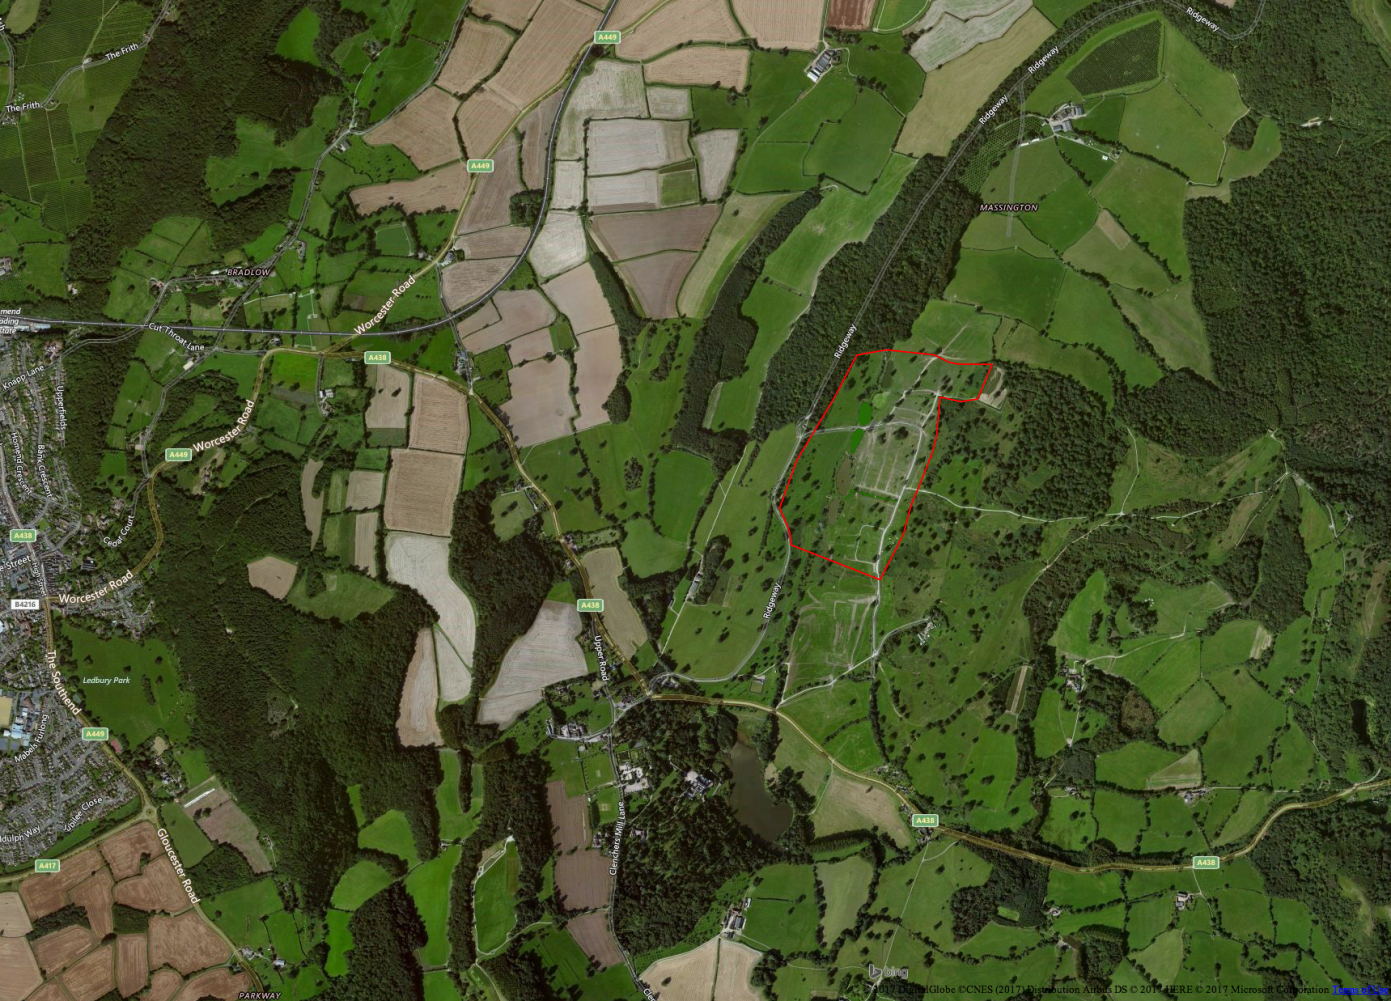
\includegraphics[width=23cm]{./supplementary/wide-map.png}
\end{landscape}

\addtocounter{subsection}{1}
\addcontentsline{toc}{subsection}{\protect\numberline{\thesubsection} Site Plan}
%%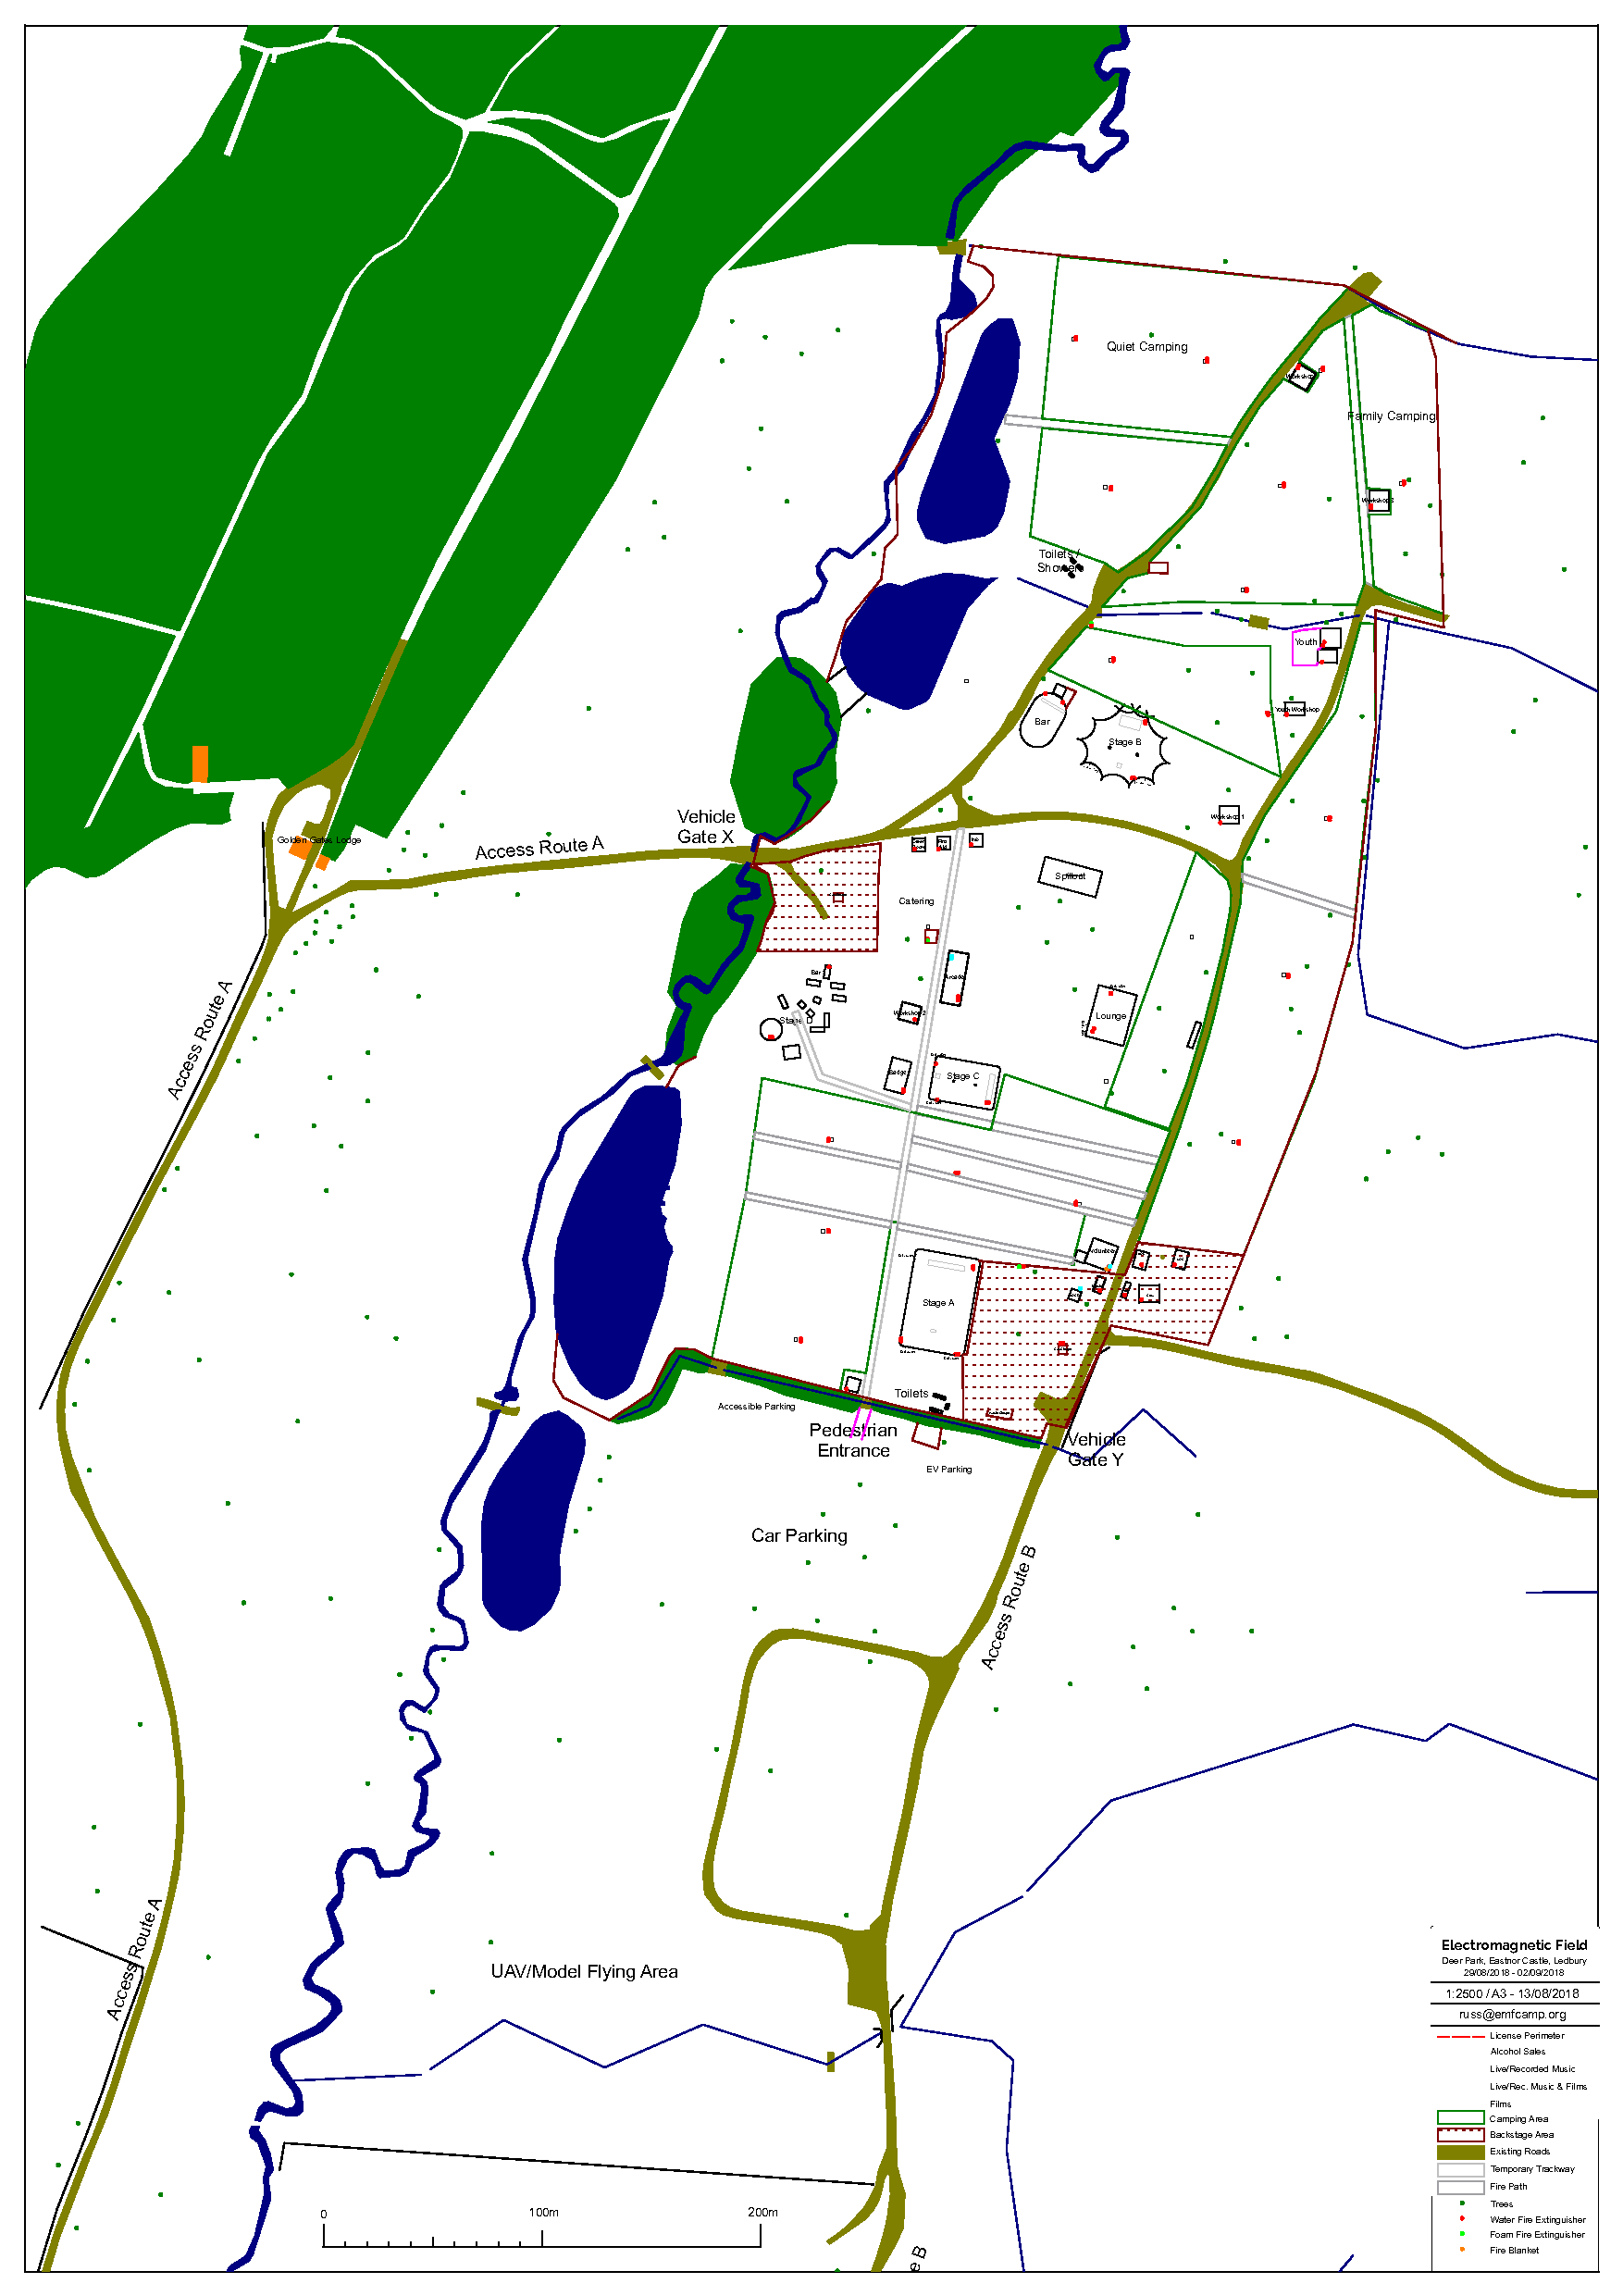
\includepdf[pages=1,fitpaper=true]{./supplementary/emf2018.pdf}
Site plan to follow.

\restoregeometry
\newpage
\begin{thebibliography}{18}
\bibitem{purpleguide}
    Events Industry Forum.
    \textit{The Purple Guide to Health, Safety and Welfare at Music and Other Events}. \\
    \href{https://www.thepurpleguide.co.uk}{https://www.thepurpleguide.co.uk}
\bibitem{bs7671}
    BSI.
    \textbf{BS 7671} \textit{Requirements for Electrical Installations. IET Wiring Regulations}.
\bibitem{bs7909}
    BSI.
    \textbf{BS 7909:2011} \textit{Code of Practice for Temporary Electrical Systems for Entertainment and Related Purposes}.
\bibitem{bs8551}
    BSI.
    \textbf{BS 8551} \textit{Provision and Management of Temporary Water Supplies}.
\bibitem{lpgsim}
    Health and Safety Executive.
    \textbf{SIM 06/2004/09} \textit{Safe Use of Liquefied Petroleum Gas (LPG) Fired Stage Flame Effects}. \\
    \href{http://www.hse.gov.uk/foi/internalops/sims/cactus/5\_04\_09.htm}{http://www.hse.gov.uk/foi/internalops/sims/cactus/5\_04\_09.htm}
\bibitem{bmflame}
    Burning Man.
    \textit{Flame Effects Guidelines}. \\
    \href{https://burningman.org/event/art-performance/fire-art-guidelines/flame-effects/}{https://burningman.org/event/art-performance/fire-art-guidelines/flame-effects/}
\bibitem{hselaser}
    Health and Safety Executive.
    \textbf{INDG224} \textit{The Safety of Laser Lighting Displays}. \\
        \href{http://www.hse.gov.uk/pubns/INDG224.htm}{http://www.hse.gov.uk/pubns/INDG224.htm}
\bibitem{plasalaser}
    PLASA.
    \textit{Safety of Display Lasers}. \\
    \href{http://www.plasa.org/technical/Laser\_Guidance.asp}{http://www.plasa.org/technical/Laser\_Guidance.asp}
\bibitem{firesafety}
    HM Government.
    \textit{Fire Safety Risk Assessment: Open Air Events and Venues}. \\
    \href{https://www.gov.uk/government/uploads/system/uploads/attachment\_data/file/14891/fsra-open-air.pdf}{https://www.gov.uk/government/uploads/system/uploads/attachment\_data/file/14891/fsra-open-air.pdf}
\bibitem{lpgstorage}
    Calor.
    \textit{Code of Guidance for the Storage of Full and Empty LPG Cylinders and Cartridges}
    \href{https://www.calor.co.uk/media/wysiwyg/PDF/code-of-guidance-for-storage-of-cylinders.pdf}{https://www.calor.co.uk/media/wysiwyg/PDF/code-of-guidance-for-storage-of-cylinders.pdf}
\bibitem{hsecrowds}
    Health and Safety Executive.
    \textbf{HSG154} \textit{Managing Crowds Safely}. \\
    \href{http://www.hse.gov.uk/pubns/books/hsg154.htm}{http://www.hse.gov.uk/pubns/books/hsg154.htm}
\bibitem{cdmguidance}
    Health and Safety Executive.
    \textit{CDM 2015 and the Entertainment Industry}. \\
    \href{http://www.hse.gov.uk/entertainment/cdm-2015/index.htm}{http://www.hse.gov.uk/entertainment/cdm-2015/index.htm}
\bibitem{istructe-tds}
    Institute of Structural Engineers.
    \textit{Temporary Demountable Structures: Guidance on procurement, design and use, third edition}.
\bibitem{mutaguide}
    MUTA.
    \textit{Best Practice Guide: Safe Use and Operation of Temporary Demountable Fabric Structures}. \\
    \href{http://www.muta.org.uk/MUTAMembers/media/MUTAMembersMedia/PDFs/MUTA-s-Best-Practice-Guide.pdf}{http://www.muta.org.uk/MUTAMembers/media/MUTAMembersMedia/PDFs/MUTA-s-Best-Practice-Guide.pdf}
\bibitem{noizcalc}
    d\&b audiotechnik.
        \textit{NoizCalc: Technical white paper (1.1 en)}. \\
    \href{http://www.dbaudio.com/en/support/downloads/category/download/7716.html}{http://www.dbaudio.com/en/support/downloads/category/download/7716.html}
\bibitem{sia}
    Security Industry Authority.
        \textit{Security at events: Guidance on the Private Security Industry Act 2001} \\
    \href{https://www.sia.homeoffice.gov.uk/Documents/licensing/sia\_security\_at\_events.pdf}{https://www.sia.homeoffice.gov.uk/Documents/licensing/sia\_security\_at\_events.pdf}
\bibitem{naru}
    National Ambulance Resilience Unit (NARU).
    \textit{National Ambulance Service Guidance for Preparing an Emergency Plan} \\
    \href{https://naru.org.uk/wp-content/uploads/2013/02/NARU-AACE-PEP-GUIDANCE-v8Fas.pdf}{https://naru.org.uk/wp-content/uploads/2013/02/NARU-AACE-PEP-GUIDANCE-v8Fas.pdf}
\end{thebibliography}
